\documentclass{article}\usepackage[]{graphicx}\usepackage[]{xcolor}
% maxwidth is the original width if it is less than linewidth
% otherwise use linewidth (to make sure the graphics do not exceed the margin)
\makeatletter
\def\maxwidth{ %
  \ifdim\Gin@nat@width>\linewidth
    \linewidth
  \else
    \Gin@nat@width
  \fi
}
\makeatother

\definecolor{fgcolor}{rgb}{0.345, 0.345, 0.345}
\newcommand{\hlnum}[1]{\textcolor[rgb]{0.686,0.059,0.569}{#1}}%
\newcommand{\hlsng}[1]{\textcolor[rgb]{0.192,0.494,0.8}{#1}}%
\newcommand{\hlcom}[1]{\textcolor[rgb]{0.678,0.584,0.686}{\textit{#1}}}%
\newcommand{\hlopt}[1]{\textcolor[rgb]{0,0,0}{#1}}%
\newcommand{\hldef}[1]{\textcolor[rgb]{0.345,0.345,0.345}{#1}}%
\newcommand{\hlkwa}[1]{\textcolor[rgb]{0.161,0.373,0.58}{\textbf{#1}}}%
\newcommand{\hlkwb}[1]{\textcolor[rgb]{0.69,0.353,0.396}{#1}}%
\newcommand{\hlkwc}[1]{\textcolor[rgb]{0.333,0.667,0.333}{#1}}%
\newcommand{\hlkwd}[1]{\textcolor[rgb]{0.737,0.353,0.396}{\textbf{#1}}}%
\let\hlipl\hlkwb

\usepackage{framed}
\makeatletter
\newenvironment{kframe}{%
 \def\at@end@of@kframe{}%
 \ifinner\ifhmode%
  \def\at@end@of@kframe{\end{minipage}}%
  \begin{minipage}{\columnwidth}%
 \fi\fi%
 \def\FrameCommand##1{\hskip\@totalleftmargin \hskip-\fboxsep
 \colorbox{shadecolor}{##1}\hskip-\fboxsep
     % There is no \\@totalrightmargin, so:
     \hskip-\linewidth \hskip-\@totalleftmargin \hskip\columnwidth}%
 \MakeFramed {\advance\hsize-\width
   \@totalleftmargin\z@ \linewidth\hsize
   \@setminipage}}%
 {\par\unskip\endMakeFramed%
 \at@end@of@kframe}
\makeatother

\definecolor{shadecolor}{rgb}{.97, .97, .97}
\definecolor{messagecolor}{rgb}{0, 0, 0}
\definecolor{warningcolor}{rgb}{1, 0, 1}
\definecolor{errorcolor}{rgb}{1, 0, 0}
\newenvironment{knitrout}{}{} % an empty environment to be redefined in TeX

\usepackage{alltt}
\usepackage[margin=1.0in]{geometry} % To set margins
\usepackage{amsmath}  % This allows me to use the align functionality.
                      % If you find yourself trying to replicate
                      % something you found online, ensure you're
                      % loading the necessary packages!
\usepackage{amsfonts} % Math font
\usepackage{fancyvrb}
\usepackage{hyperref} % For including hyperlinks
\usepackage[shortlabels]{enumitem}% For enumerated lists with labels specified
                                  % We had to run tlmgr_install("enumitem") in R
\usepackage{float}    % For telling R where to put a table/figure
\usepackage{natbib}        %For the bibliography
\bibliographystyle{apalike}%For the bibliography
\IfFileExists{upquote.sty}{\usepackage{upquote}}{}
\begin{document}


\cite{Kasdin25} show that dopamine in the brains of young zebra finches acts as 
a learning signal, increasing when they sing closer to their adult song and 
decreasing when they sing further away, effectively guiding their vocal 
development through trial-and-error. This suggests that complex natural 
behaviors, like learning to sing, are shaped by dopamine-driven reinforcement 
learning, similar to how artificial intelligence learns. You can find the 
paper at this link:
\href{https://www.nature.com/articles/s41586-025-08729-1}{{https://www.nature.com/articles/s41586-025-08729-1}.}.

Note they measure dopamine using fibre photometry, changes in the fluorescence
indicate dopamine changes in realtime. Their specific measurement considers 
changes in flourescence in 100-ms windows between 200 and 300 ms from the start 
of singing, averaged across development.

\begin{enumerate}
%%%%%%%%%%%%%%%%%%%%%%%%%%%%%%%%%%%%%%%%%%%%%%%%%%%%%%%%%%%%%%%%%
% CONDUCT A POWER ANALYSIS
%%%%%%%%%%%%%%%%%%%%%%%%%%%%%%%%%%%%%%%%%%%%%%%%%%%%%%%%%%%%%%%%%
\item Using the \texttt{pwr} package for \texttt{R} \citep{pwr},
conduct a power analysis. How many observations would the researchers 
need to detect a moderate-to-large effect ($d=0.65$) when using 
$\alpha=0.05$ and default power (0.80) for a two-sided one sample 
$t$ test.
\begin{knitrout}\scriptsize
\definecolor{shadecolor}{rgb}{0.969, 0.969, 0.969}\color{fgcolor}\begin{kframe}


{\ttfamily\noindent\color{warningcolor}{\#\# Warning: package 'pwr' was built under R version 4.4.3}}\end{kframe}
\end{knitrout}
\begin{knitrout}\scriptsize
\definecolor{shadecolor}{rgb}{0.969, 0.969, 0.969}\color{fgcolor}\begin{kframe}
\begin{alltt}
\hlkwd{pwr.t.test}\hldef{(}
  \hlkwc{d} \hldef{=} \hlnum{0.65}\hldef{,}
  \hlkwc{sig.level} \hldef{=} \hlnum{0.05}\hldef{,}
  \hlkwc{power} \hldef{=} \hlnum{0.80}\hldef{,}
  \hlkwc{type} \hldef{=} \hlsng{"one.sample"}\hldef{,}
  \hlkwc{alternative} \hldef{=} \hlsng{"two.sided"}
\hldef{)}
\end{alltt}
\begin{verbatim}
## 
##      One-sample t test power calculation 
## 
##               n = 20.58039
##               d = 0.65
##       sig.level = 0.05
##           power = 0.8
##     alternative = two.sided
\end{verbatim}
\end{kframe}
\end{knitrout}
Using the \verb|pwr.t.test()| function indicates that we need 21 obervations.

%%%%%%%%%%%%%%%%%%%%%%%%%%%%%%%%%%%%%%%%%%%%%%%%%%%%%%%%%%%%%%%%%
% COLLECT DATA
%%%%%%%%%%%%%%%%%%%%%%%%%%%%%%%%%%%%%%%%%%%%%%%%%%%%%%%%%%%%%%%%%
\item Click the link to go to the paper. Find the source data for 
Figure 2. Download the Excel file. Describe what you needed to
do to collect the data for Figure 2(g). Note that you only need the 
\texttt{closer\_vals} and \texttt{further\_vals}. Ensure to 
\texttt{mutate()} the data to get a difference 
(e.g., \texttt{closer\_vals - further\_vals}).

In order to collect \texttt{closer\_vals} and \texttt{further\_vals} from the excel file I had to manual go through the file and copy and paste both of those columns of values onto a new excel page. Once I had the data on a new excel file I then renamed the columns using the \verb|rename()| function and use mutate to create the difference. 
%%%%%%%%%%%%%%%%%%%%%%%%%%%%%%%%%%%%%%%%%%%%%%%%%%%%%%%%%%%%%%%%%
% SUMMARIZE DATA
%%%%%%%%%%%%%%%%%%%%%%%%%%%%%%%%%%%%%%%%%%%%%%%%%%%%%%%%%%%%%%%%%
\item Summarize the data.
\begin{enumerate}
  \item Summarize the further data. Do the data suggest that
   dopamine in the brains of young zebra finches decreases when
   they sing further away?
\begin{table}[ht]
\centering
\begin{tabular}{rrrrrr}
  \hline
mean & sd & median & min & max \\ 
  \hline
-0.20 & 0.13 & -0.19 & -0.60 & -0.03 \\ 
   \hline
\end{tabular}
\end{table}
   
The mean dopamine response when zebra finches sang farther from their adult songs was -0.20 with a standard deviation of 0.13 which may indicate a decrease in dopamine. The responses ranged from -.60 to -.03 which tell us that all of our observed values indicated that singing farther away from their adult songs had a negative impact on their dopamine levels. We can also look to Figure \ref{plot1} which visual shows us that all of our obersvations are recorded below zero and our median is well below zero indicating a negative effect.  
   
   \item Summarize the closer data. Do the data suggest that
   dopamine in the brains of young zebra finches increases when
   they sing closer to their adult song?
 \begin{table}[ht]
\centering
\begin{tabular}{rrrrrr}
  \hline
mean & sd & median & min & max \\ 
  \hline
0.16 & 0.09 & 0.15 & 0.00 & 0.34 \\ 
   \hline
\end{tabular}
\end{table}
   
   The mean dopamine response when zebra finches sang closer to their adult songs was 0.16 with a standard deviation of 0.09 which may indicate a increase in dopamine. The responses ranged from 0 to .34 which tell us that all of our observed values indicated that singing closer to their adult songs had a positive impact on their dopamine levels. We can also look to Figure \ref{plot1} which visual shows us that all of our obersvations are recorded at or above zero and are median is well above zero again, indicating a postive effect. 
   
   
  \item Summarize the paired differences. Do the data suggest
  that there is a difference between dopamine in the brains of
  young zebra finches when they sing further away compared to 
  closer to their adult song?
\begin{table}[ht]
\centering
\begin{tabular}{rrrrrr}
  \hline
mean & sd & median & min & max \\ 
  \hline
0.36 & 0.21 & 0.33 & 0.04 & 0.93 \\ 
   \hline
\end{tabular}
\end{table}

Taking the difference for each bird allows us to control for variability in baseline dopamine levels and assess the direct effect that singing closer or farther from their adult song might have on their dopamine levels. Given this we see that the mean difference between closer and farther dopamine levels is .36. Our data indicate that the zebra finches showed higher dopamine levels when singing closer to their adult song compared to when they sing further away. We can again visual see this in Figure \ref{plot1} which reinforces our numerical summary of our data and our original conclusion. 

  
  \begin{figure}[H]
  \begin{center}
  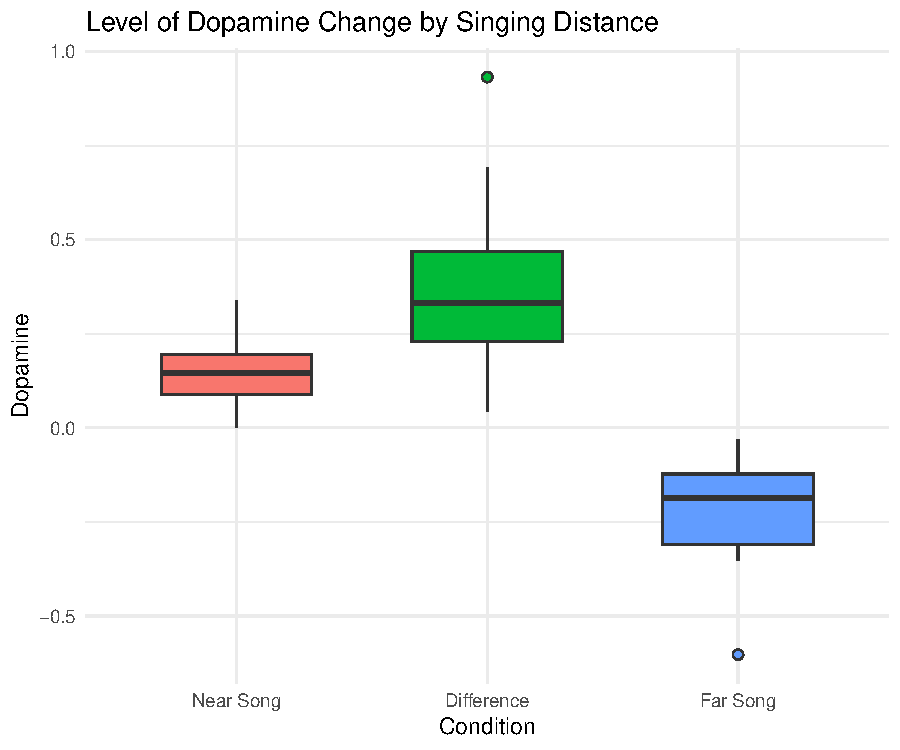
\includegraphics[scale=.8]{boxplot.finchdat.pdf}
  \caption{Box Plot of Dopmaine in Zebra Finches}
  \label{plot1}
  \end{center}
\end{figure}
  
  \newpage
  
  \item \textbf{Optional Challenge:} Can you reproduce Figure 2(g)?
  Note that the you can use \texttt{geom\_errorbar()} to plot
  the range created by adding the mean $\pm$ one standard deviation.
  
 \begin{figure}[H]
  \begin{center}
  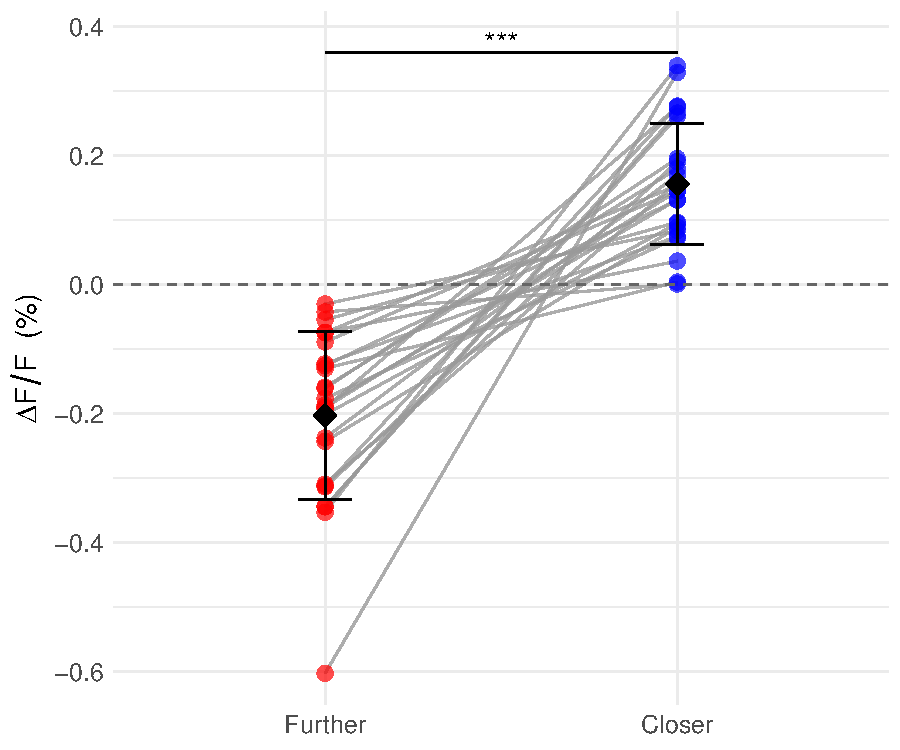
\includegraphics[scale=.8]{optionalgraph.pdf}
  \caption{optional graph}
  \label{plot2}
  \end{center}
\end{figure} 

\end{enumerate}
%%%%%%%%%%%%%%%%%%%%%%%%%%%%%%%%%%%%%%%%%%%%%%%%%%%%%%%%%%%%%%%%%
% CONDUCT THE TESTS
%%%%%%%%%%%%%%%%%%%%%%%%%%%%%%%%%%%%%%%%%%%%%%%%%%%%%%%%%%%%%%%%%
\newpage
\item Conduct the inferences they do in the paper. Make sure to report the results
a little more comprehensively -- that is your parenthetical should look something
like: ($t=23.99$, $p<0.0001$; $g=1.34$; 95\% CI: 4.43, 4.60).\\
\textbf{Note:} Your numbers may vary slightly as they performed some unclear
correction of their $p$-values. I'm waiting to hear back from them via email!
\begin{enumerate}
  \item ``The close responses differed significantly from 0 ($t=8.3$, p$\leq$0.0001; g=1.61; 95\% CI: 0.12, 0.2)."
  
  \item ``The far responses differed significantly from 0 ($t=-7.78$, p$\leq$0.0001; g=-1.51; 95\% CI: -0.26, -0.15)."
  
  \item ``The difference between populations was significant ($t=8.51$, p$\leq$0.0001; g=1.65; 95\% CI: 0.27, 0.45)."
\end{enumerate}

Each of the above parentheticals are from the two tailed test.
%%%%%%%%%%%%%%%%%%%%%%%%%%%%%%%%%%%%%%%%%%%%%%%%%%%%%%%%%%%%%%%%%
% CONDUCT THE TESTS
%%%%%%%%%%%%%%%%%%%%%%%%%%%%%%%%%%%%%%%%%%%%%%%%%%%%%%%%%%%%%%%%%
\item Reverse engineer the hypothesis test plot from Lecture 20 to create accurate
hypothesis testing plots for each part of the previous question.
\begin{enumerate}
  \item Question 4, part(a).
   \begin{figure}[H]
  \begin{center}
  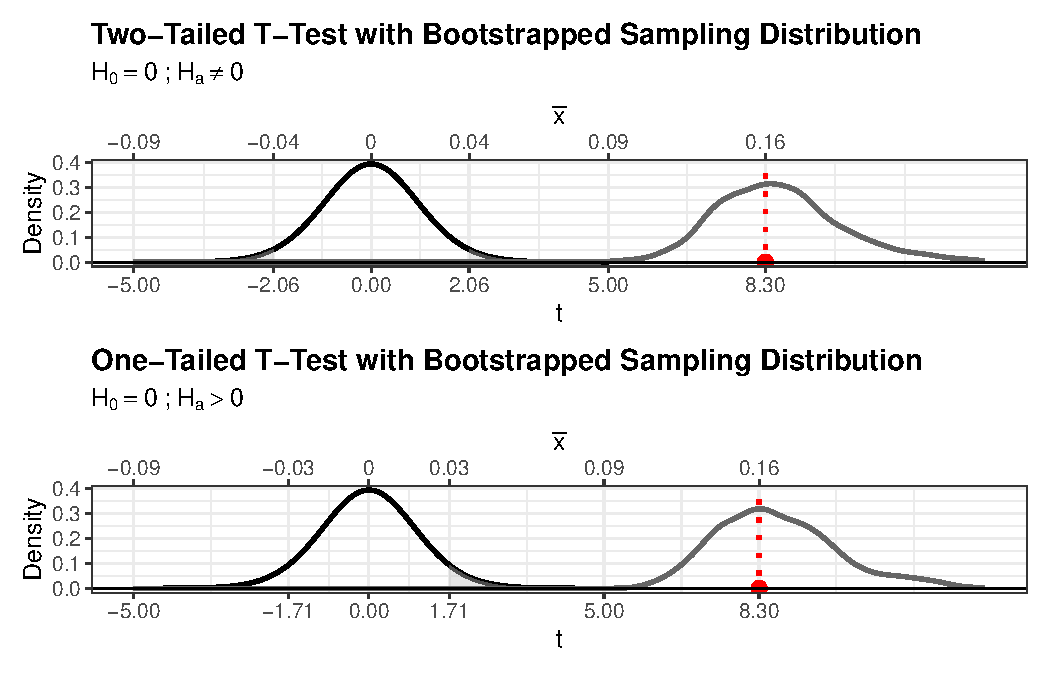
\includegraphics[scale=.8]{close.hyp.plots.pdf}
  \caption{Two-tailed and one-tailed hypothesis tests for dopamine levels when singing closer to the adult song}
  \label{plot3}
  \end{center}
\end{figure} 

\newpage

  \item Question 4, part(b).
   \begin{figure}[H]
  \begin{center}
  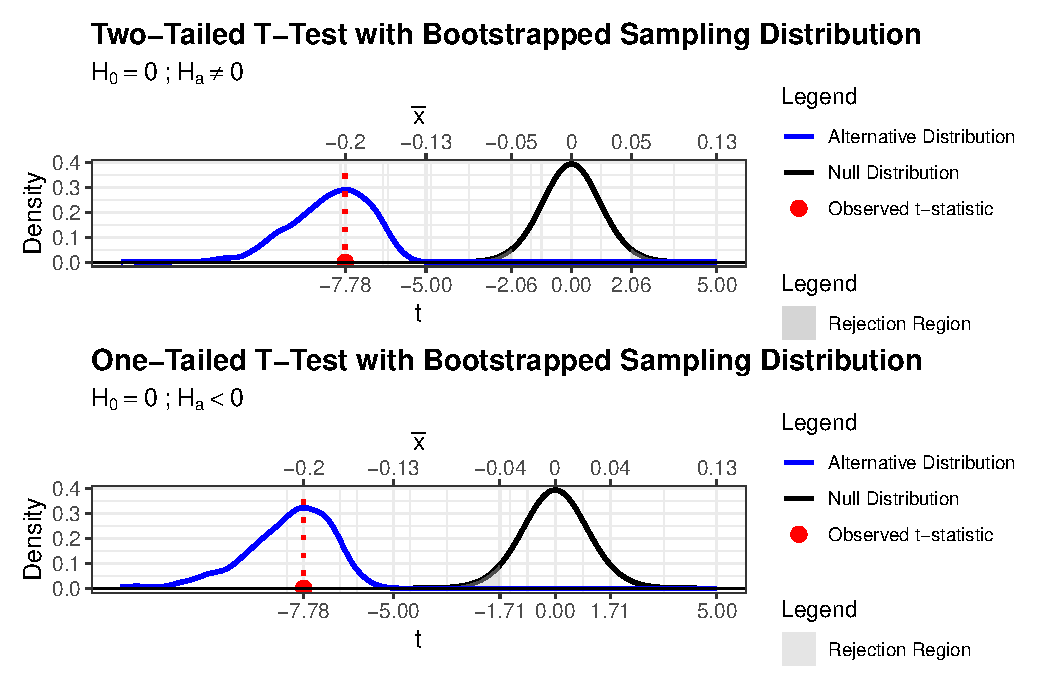
\includegraphics[scale=.8]{farther.hyp.plots.pdf}
  \caption{Two-tailed and one-tailed hypothesis tests for dopamine levels when singing farther from the adult song}
  \label{plot4}
  \end{center}
\end{figure} 
  
\newpage  
  \item Question 4, part(c).
   \begin{figure}[H]
  \begin{center}
  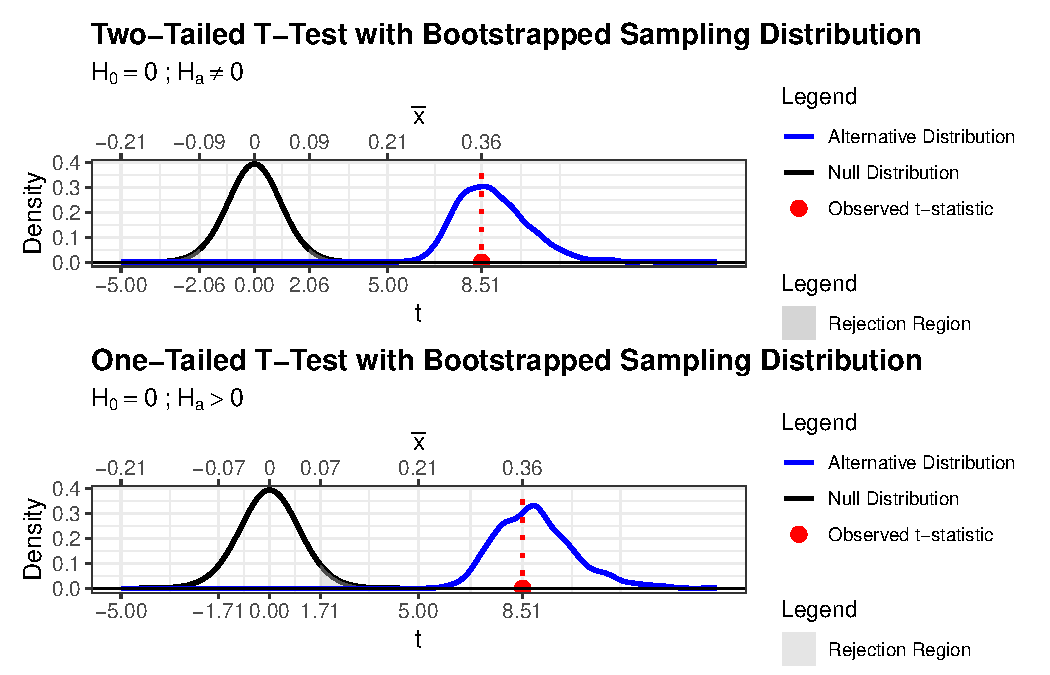
\includegraphics[scale=.8]{diff.hyp.plots.pdf}
  \caption{Two-tailed and one-tailed hypothesis tests for the difference in dopamine levels between close and far singing conditions}
  \label{plot5}
  \end{center}
\end{figure} 
\end{enumerate}
\end{enumerate}


\bibliography{bibliography}
\end{document}
